Considérons que nous cherchons de manière empirique à obtenir des connaissances sur l'aire de base et le volume des formes géométriques tridimensionelles \marginnote{Le code de cet exemple est disponible à cette adresse \url{}}.

La création de l'expérimentation \textsl{geometricShape} se fait comme suit :
\mcode{expCreate('geometricShape');}
Nous pouyvons ensuite instnatier deux étapes de traitement, une qui se chargera du calcul de l'aire de la base:
\mcode{geometricShape('addStep', 'base');}
et une autre du volume :
\mcode{geometricShape('addStep', 'space');}
Nous nous intéressons à l'influence potentielle des différents attributs (forme, couleur, rayon, largeur, hauteur) sur l'aire de sa base et son volume. Nous considérons donc chacun de ces attributs comme des facteur expérimentaux avec des modalités données.

Les formes étudiées sont le cylindre, la pyramide et le cube :
\begin{lstlisting}
geometricShape('addFactor', ...
	{'shape', {'cylinder', 'pyramid', 'cube'}});
\end{lstlisting}
La couleur peut être bleu ou rouge, le rayon peut être de 2, 4, ou 6 mètres, la largeur de la pyramide et du cube peut être de 1, 2, et 3 mètres et la hauteur de 2, 4 ,et 6 mètres. On note ici une exclusion qui est courante dans tout plan expérimental de complexité raisonnable avec plusieurs approches mise en compétition, certains facteurs ne devront être explorés que pour une modalité d'un autre facteur.
\begin{lstlisting}
geometricShape('addFactor', {'color', {'blue', 'red'}});
geometricShape('addFactor', {'radius', '[2, 4, 6]', '', '1/1'});
geometricShape('addFactor', {'width', '1:3', '', '1/[2 3]'});
geometricShape('addFactor', {'height', '2:2:6', '2', '1/[1 2]'});
\end{lstlisting}
Cette série de commandes permet de spécifier le plan expérimental, disponible dans le fichier \mcode{geshFactors.txt} :
\begin{lstlisting}
Factors:
1    shape =  =  = {'cylinder', 'pyramid', 'cube'}
2    color =  =  = {'blue', 'red'}
3    radius =  = 1/1 = [2, 4, 6]
4    width =  = 1/[2 3] = 1:3
5    height = 2 = 1/[1 2] = 2:2:6
\end{lstlisting}
La ligne 5 peut se lire comme suit, le facteur "height" n'est pertinent que pour l'étape 2 et les modalités 1 et 2 du facteur 1.

Les deux étapes de traitement sont implantées comme suit :
\begin{lstlisting}

\end{lstlisting}
Chaque étape dispose de la même signature, la variable variable \textsl{config} expose la configuration de l'expérimentation, la variable \textsl{data} expose les données produite par l'étape précédente ou les données d'entrée pour la première étape, et la variable \textsl{setting} la condition expérimentale courante. 

\subsection{Implement processing steps}

The first step is dedicated to the computation of the base area of the shape. The solution code is implemented in \mcode{gesh1base.m}, where we simulate that $\pi$ is estimated with a given precision, but 100 measurements have been made:
\lstinputlisting[firstline=16, lastline=23]{../demo/geometricShape/gesh1base.m}


The second step builds upon the result of the first processing step to compute the volume (implemented in \mcode{gesh2volume.m}):
\lstinputlisting[firstline=16, lastline=23]{../demo/geometricShape/gesh2space.m}

\subsection{Define observations}

Observations for the 2 processing steps are the following. First step:
\lstinputlisting[firstline=24, lastline=24]{../demo/geometricShape/gesh1base.m}
Second step:
\lstinputlisting[firstline=25, lastline=26]{../demo/geometricShape/gesh2space.m}

\begin{marginfigure}
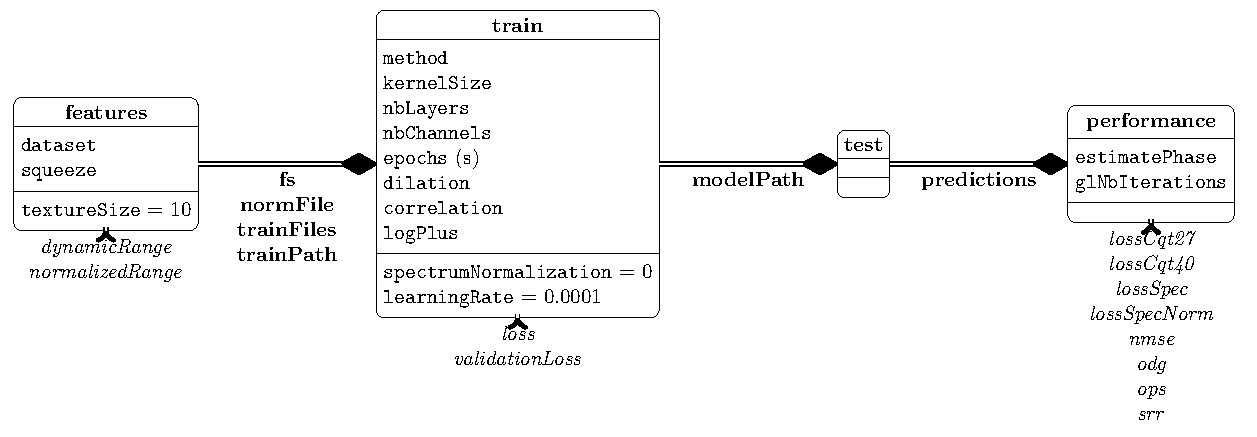
\includegraphics[width=1.2\textwidth]{../demo/geometricShape/report/figures/factors}
\end{marginfigure}

The command \mcode{geometricShape('f')} generates a diagram view of the experiment.

\subsection{Process}

\begin{lstlisting}
geometricShape('do', 1);
\end{lstlisting}
run the base step over all 18 settings.
\begin{lstlisting}
geometricShape('do', 0, 'mask', {[1 2] 0 1});
\end{lstlisting}
runs successively each step over the cylinders of radius 2 and all the pyramids.

\subsection{Expose observations}

\begin{marginfigure}
\includegraphics[trim={0 6cm 0 0},clip,width=1.2\textwidth]{../demo/geometricShape/report/figures/mtable}
\end{marginfigure}

Upon completion of the processing, the results of the last processing are displayed in the command window:

This display can be obtained by issuing the following command:
\begin{lstlisting}
geometricShape('display', 2, 'expose', '>', ...
	'mask', {[1 2] 0 1});
\end{lstlisting}
The exposition of relevant observations is important for efficient computational experimentation. \explanes provides many tools for this purpose, type \mcode{help expExpose} for quick reference.


The command:
\begin{lstlisting}
geometricShape('display', 2, 'mask', {1 0 1},...
 'expose', {'t', 'obs', 3, 'sort', 1});
\end{lstlisting}

displays the volume (observation 3) of the step volume (2) for each cylinder of radius 2 sorted according to the first on a table (t). Red color indicates best performance, and blue ones, performances which have not been found statistically different from the best one.
\marginnote{For this example, even if the blue cylinder is bigger than the red one due to the uncertainty in the estimation of $\pi$, this difference is not significant, so the blue and red cylinders shall be considered of equivalent volume.}

\subsection{Report}

\begin{margintable}
\caption{\latex table output.}
\input{../demo/geometricShape/report/tables/geolTabular}
\end{margintable}

The file \mcode{<shortExperimentName>Report.m}, that is \mcode{geshReport.m} in this example, allows you to generate a report that compiles several expositions of observations: \LaTeX table (l), bar plot (b), and box plot (x).

\lstinputlisting[firstline=13, lastline=19]{../demo/geometricShape/geshReport.m}

\begin{marginfigure}
\includegraphics[width=\textwidth]{../demo/geometricShape/report/figures/geob}
\end{marginfigure}


\begin{marginfigure}
\includegraphics[width=\textwidth]{../demo/geometricShape/report/figures/geox}
\end{marginfigure}


Several reports can be handled for the same experiment using the key \mcode{'reportName'}, and if the name of the report contain the key \mcode{'Slides'}, a slide presentation layout is used. For example, the command:
\begin{lstlisting}
geometricShape('report', 'rcv', ...
  'reportName', 'presentationSlides');
\end{lstlisting}
generates a report with base name \mcode{presentationSlides} in a slides presentation layout. For debug information about the compilation, please add the \mcode{'b'} flag to the \mcode{report} value.
